\documentclass[a4paper, 12pt]{article}\usepackage[]{graphicx}\usepackage[]{color}
%% maxwidth is the original width if it is less than linewidth
%% otherwise use linewidth (to make sure the graphics do not exceed the margin)
\makeatletter
\def\maxwidth{ %
  \ifdim\Gin@nat@width>\linewidth
    \linewidth
  \else
    \Gin@nat@width
  \fi
}
\makeatother

\definecolor{fgcolor}{rgb}{0.345, 0.345, 0.345}
\newcommand{\hlnum}[1]{\textcolor[rgb]{0.686,0.059,0.569}{#1}}%
\newcommand{\hlstr}[1]{\textcolor[rgb]{0.192,0.494,0.8}{#1}}%
\newcommand{\hlcom}[1]{\textcolor[rgb]{0.678,0.584,0.686}{\textit{#1}}}%
\newcommand{\hlopt}[1]{\textcolor[rgb]{0,0,0}{#1}}%
\newcommand{\hlstd}[1]{\textcolor[rgb]{0.345,0.345,0.345}{#1}}%
\newcommand{\hlkwa}[1]{\textcolor[rgb]{0.161,0.373,0.58}{\textbf{#1}}}%
\newcommand{\hlkwb}[1]{\textcolor[rgb]{0.69,0.353,0.396}{#1}}%
\newcommand{\hlkwc}[1]{\textcolor[rgb]{0.333,0.667,0.333}{#1}}%
\newcommand{\hlkwd}[1]{\textcolor[rgb]{0.737,0.353,0.396}{\textbf{#1}}}%
\let\hlipl\hlkwb

\usepackage{framed}
\makeatletter
\newenvironment{kframe}{%
 \def\at@end@of@kframe{}%
 \ifinner\ifhmode%
  \def\at@end@of@kframe{\end{minipage}}%
  \begin{minipage}{\columnwidth}%
 \fi\fi%
 \def\FrameCommand##1{\hskip\@totalleftmargin \hskip-\fboxsep
 \colorbox{shadecolor}{##1}\hskip-\fboxsep
     % There is no \\@totalrightmargin, so:
     \hskip-\linewidth \hskip-\@totalleftmargin \hskip\columnwidth}%
 \MakeFramed {\advance\hsize-\width
   \@totalleftmargin\z@ \linewidth\hsize
   \@setminipage}}%
 {\par\unskip\endMakeFramed%
 \at@end@of@kframe}
\makeatother

\definecolor{shadecolor}{rgb}{.97, .97, .97}
\definecolor{messagecolor}{rgb}{0, 0, 0}
\definecolor{warningcolor}{rgb}{1, 0, 1}
\definecolor{errorcolor}{rgb}{1, 0, 0}
\newenvironment{knitrout}{}{} % an empty environment to be redefined in TeX

\usepackage{alltt}
\usepackage[utf8]{inputenc}
\usepackage[brazilian, english]{babel}
\usepackage{indentfirst}
\usepackage{graphicx}
\usepackage{float}
\usepackage{titlesec}
\usepackage{amsmath}
\usepackage{caption}
\usepackage{subfigure}
\usepackage{hyperref}
%\usepackage{fixltx2e} %Para subscripts
\usepackage{pgfplots}
\usepackage{textcomp}
\usepackage{enumitem}
\usepackage{multicol}


\title{\textbf{Tooth Growth, Vitamin C and Orange Juice - A Statistical Approach}}
\author{\textit{Eric Calasans de Barros}}
\IfFileExists{upquote.sty}{\usepackage{upquote}}{}
\begin{document}
        \section{Introduction}
        In this paper we want study the influence of vitamin C ingest in teeth growth applying some statistical techniques.
        
        \section{Metodology}
        \subsection{Loading Data}
        First we load the ToothGrowt dataset from \texttt{dataset} library in R and the others necessary libraries.  Here's the code:
\begin{knitrout}\small
\definecolor{shadecolor}{rgb}{0.969, 0.969, 0.969}\color{fgcolor}\begin{kframe}
\begin{alltt}
\hlkwd{library}\hlstd{(datasets)}
\hlkwd{library}\hlstd{(ggplot2)}
\hlkwd{library}\hlstd{(dplyr)}
\end{alltt}


{\ttfamily\noindent\color{warningcolor}{\#\# Warning: package 'dplyr' was built under R version 3.4.2}}\begin{alltt}
\hlstd{TG} \hlkwb{<-} \hlkwd{data.frame}\hlstd{(ToothGrowth)}
\end{alltt}
\end{kframe}
\end{knitrout}
        \subsection{Exploratory Data Analysis}
        Next, we can take a look at the data structure, contents and statistical elements such as mean, min, max, etc.
\begin{knitrout}\small
\definecolor{shadecolor}{rgb}{0.969, 0.969, 0.969}\color{fgcolor}\begin{kframe}
\begin{alltt}
\hlkwd{str}\hlstd{(TG)}
\end{alltt}
\begin{verbatim}
## 'data.frame':	60 obs. of  3 variables:
##  $ len : num  4.2 11.5 7.3 5.8 6.4 10 11.2 11.2 5.2 7 ...
##  $ supp: Factor w/ 2 levels "OJ","VC": 2 2 2 2 2 2 2 2 2 2 ...
##  $ dose: num  0.5 0.5 0.5 0.5 0.5 0.5 0.5 0.5 0.5 0.5 ...
\end{verbatim}
\begin{alltt}
\hlkwd{head}\hlstd{(TG)}
\end{alltt}
\begin{verbatim}
##    len supp dose
## 1  4.2   VC  0.5
## 2 11.5   VC  0.5
## 3  7.3   VC  0.5
## 4  5.8   VC  0.5
## 5  6.4   VC  0.5
## 6 10.0   VC  0.5
\end{verbatim}
\begin{alltt}
\hlkwd{summary}\hlstd{(TG)}
\end{alltt}
\begin{verbatim}
##       len        supp         dose      
##  Min.   : 4.20   OJ:30   Min.   :0.500  
##  1st Qu.:13.07   VC:30   1st Qu.:0.500  
##  Median :19.25           Median :1.000  
##  Mean   :18.81           Mean   :1.167  
##  3rd Qu.:25.27           3rd Qu.:2.000  
##  Max.   :33.90           Max.   :2.000
\end{verbatim}
\end{kframe}
\end{knitrout}
	We can observe that the dataset is composed by 3 variables:
	\begin{itemize}
		\item \texttt{len} - tooth length(numerical);
		\item \texttt{supp} - a factor indicating Orange Juice(OJ) or Vitamin C(VC);
		\item \texttt{dose} - dose(mg).		
	\end{itemize}
	
	Here we have some exploratory data analysis in the dataset.  First, to make easy for plotting, we convert \texttt{dose} to a factor variable because there are only three kind of quantity:
\begin{knitrout}\small
\definecolor{shadecolor}{rgb}{0.969, 0.969, 0.969}\color{fgcolor}\begin{kframe}
\begin{alltt}
\hlstd{TG} \hlkwb{<-} \hlkwd{mutate}\hlstd{(TG,} \hlkwc{dose} \hlstd{=} \hlkwd{as.factor}\hlstd{(dose))}
\end{alltt}
\end{kframe}
\end{knitrout}
  We can make somoe plots and see what we can find:
\begin{knitrout}\small
\definecolor{shadecolor}{rgb}{0.969, 0.969, 0.969}\color{fgcolor}\begin{kframe}
\begin{alltt}
\hlstd{g1} \hlkwb{<-} \hlkwd{ggplot}\hlstd{(TG,} \hlkwd{aes}\hlstd{(}\hlkwc{x}\hlstd{=dose,} \hlkwc{y}\hlstd{=len,} \hlkwc{fill}\hlstd{=supp))}
\hlstd{g1} \hlkwb{<-} \hlstd{g1} \hlopt{+} \hlkwd{geom_boxplot}\hlstd{()} \hlopt{+} \hlkwd{facet_grid}\hlstd{(.}\hlopt{~}\hlstd{supp)}
\hlstd{g1} \hlkwb{<-} \hlstd{g1} \hlopt{+} \hlkwd{ggtitle}\hlstd{(}\hlstr{"Tooth Growth x Dose x Supp Type"}\hlstd{)}
\hlstd{g1} \hlkwb{<-} \hlstd{g1} \hlopt{+} \hlkwd{labs}\hlstd{(}\hlkwc{x} \hlstd{=} \hlstr{"Dose(mg)"}\hlstd{,} \hlkwc{y} \hlstd{=} \hlstr{"Teeth Length"}\hlstd{)}
\hlstd{g1} \hlkwb{<-} \hlstd{g1} \hlopt{+} \hlkwd{guides}\hlstd{(}\hlkwc{fill}\hlstd{=}\hlkwd{guide_legend}\hlstd{(}\hlstr{"Supp type"}\hlstd{))}
\hlstd{g1}
\end{alltt}
\end{kframe}

{\centering 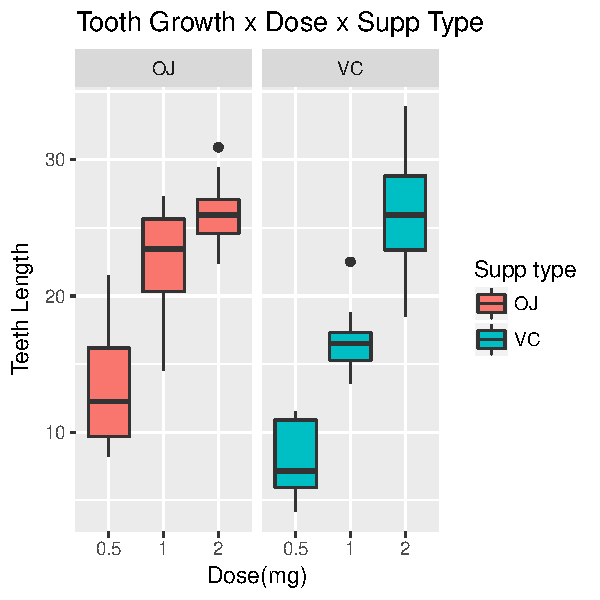
\includegraphics[width=\maxwidth]{figure/plot1-1} 

}



\end{knitrout}

As far we can observe, when dose increases the tooth length increases too, no matter what kind of supplement is given.  Now let's compare supplement type closely.
\begin{knitrout}\small
\definecolor{shadecolor}{rgb}{0.969, 0.969, 0.969}\color{fgcolor}\begin{kframe}
\begin{alltt}
\hlstd{g2} \hlkwb{<-} \hlkwd{ggplot}\hlstd{(TG,} \hlkwd{aes}\hlstd{(}\hlkwc{x}\hlstd{=supp,} \hlkwc{y}\hlstd{=len,} \hlkwc{fill}\hlstd{=supp))}
\hlstd{g2} \hlkwb{<-} \hlstd{g2} \hlopt{+} \hlkwd{geom_boxplot}\hlstd{(}\hlkwd{aes}\hlstd{(}\hlkwc{fill}\hlstd{=supp))} \hlopt{+} \hlkwd{facet_wrap}\hlstd{(}\hlopt{~} \hlstd{dose)}
\hlstd{g2} \hlkwb{<-} \hlstd{g2} \hlopt{+} \hlkwd{ggtitle}\hlstd{(}\hlstr{"Tooth Growth x Dose x Supp Type"}\hlstd{)}
\hlstd{g2} \hlkwb{<-} \hlstd{g2} \hlopt{+} \hlkwd{labs}\hlstd{(}\hlkwc{x} \hlstd{=} \hlstr{"Dose(mg)"}\hlstd{,} \hlkwc{y} \hlstd{=} \hlstr{"Teeth Length"}\hlstd{)}
\hlstd{g2} \hlkwb{<-} \hlstd{g2} \hlopt{+} \hlkwd{guides}\hlstd{(}\hlkwc{fill}\hlstd{=}\hlkwd{guide_legend}\hlstd{(}\hlstr{"Supp type"}\hlstd{))}
\hlstd{g2}
\end{alltt}
\end{kframe}

{\centering 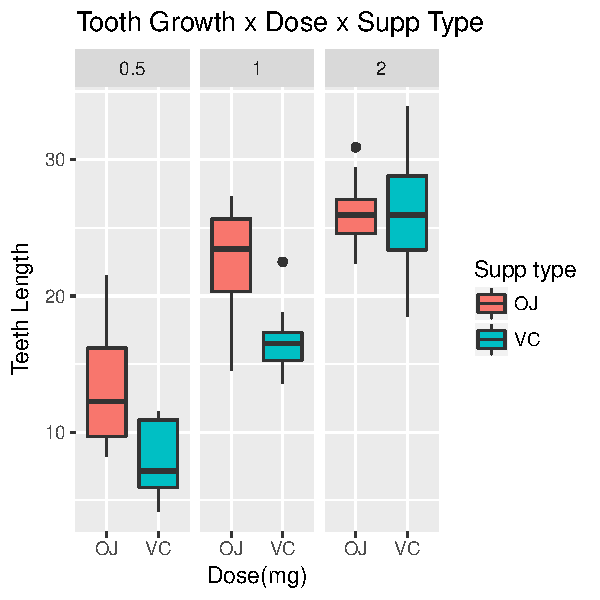
\includegraphics[width=\maxwidth]{figure/plot2-1} 

}



\end{knitrout}

In this plot we can see that low doses of OJ increases tooth growth comparing with VC, which is as effective as OJ in higher doses.

        \subsection{Hypotesis Test}
        Hypotesis Tests are a powerful tool in data analysis when we want achieve statistical support for certain statements.  For this dataset we want verify influence of kind of supplement and dose amount in tooth growth in a more detailed way.  We will test first if kind of supplement influences tooth growth and after that, given one of the doses if one or more is involved in incresase of growth.\\
        
        For this purpose, given the fact that we don't know population mean and population variance, the \textbf{t-test} is indicated.
\end{document}


